%% ============================================================
%% Finance Research Letters submission
%% Chronotypic Market Ecology
%% Subramanian & Seetharaman (2026)
%% Target: <2500 words main text (excl. abstract, refs, tables,
%%          figures, captions, acknowledgements, declarations,
%%          appendices).
%% ============================================================

\documentclass[preprint,12pt,authoryear]{elsarticle}

\usepackage{amsmath,amssymb,amsthm}
\usepackage{booktabs}
\usepackage{lineno}
\usepackage{url}
\usepackage[expansion=false]{microtype}

\graphicspath{{figures/}}

\newtheorem{theorem}{Theorem}
\newtheorem{definition}{Definition}
\newtheorem{remark}{Remark}

\journal{Finance Research Letters}

\begin{document}

\linenumbers

\begin{frontmatter}

\title{Chronotypic Market Ecology: Temporal Homophily,
       Network Fragmentation, and Market Stability}

\author[vchs]{Sanjay Subramanian\corref{cor1}}
\ead{jaysubbu@gmail.com}

\author[vchs]{Sumedh Seetharaman}

\cortext[cor1]{Corresponding author.}

\affiliation[vchs]{organization={Valley Christian High School},
             addressline={100 Skyway Drive},
             city={San Jose},
             postcode={95138},
             state={CA},
             country={USA}}

%% -------------------------------------------------------
\begin{abstract}
We introduce Chronotypic Market Ecology (CME), an agent-based framework
in which market participants are characterised by their temporal scale
$\tau$---the lookback horizon over which they evaluate price signals.
Agents with similar $\tau$ preferentially form trade relationships
(\emph{temporal homophily}, strength $\kappa_h$), creating an endogenous
$\tau$-proximity network whose topology shapes price dynamics.
Using a calibrated simulation (four investor types from 2023 AUM data,
$n = 80$, $T = 500$, 250 runs) we establish three results that together
constitute a network-based microfoundation for the Fractal Market
Hypothesis \citep{peters1994}: homophily is a \emph{dual-channel} force
that stabilises prices in the short run while sowing the conditions for
long-run instability.
First, increasing homophily suppresses aggregate return volatility
($1.29\times$, $t = 15.1$, $p < 10^{-20}$) by reducing cross-$\tau$
friction---the short-run stabilising channel.
Second, the Temporal Market Fragmentation Index (TMFI) falls $14.28\times$
versus only $1.29\times$ for volatility, nearly eliminating temporal
fragmentation as $\tau$-communities converge.
Third, $\tau$-adaptation is self-reinforcing under high homophily
($\Delta\mathrm{TDI} = -0.114$ at $\kappa_h = 3.0$ over ten cycles),
producing temporal echo chambers that compress the horizon diversity the
FMH identifies as the foundation of market stability---the long-run
destabilising channel.
Empirical validation using SEC Form~13-F institutional holdings
(2013 Q3--2024 Q3, $n = 45$ quarters with $\geq 50$ reporting
institutions) yields $r(\mathrm{TDI}, \mathrm{VIX}) = -0.526$
($p < 0.001$), consistent with the long-run channel.
\end{abstract}

%% -------------------------------------------------------
\begin{highlights}
\item Agent-based model of temporal heterogeneity in financial markets (CME)
\item Temporal homophily suppresses volatility 1.29$\times$ and fragmentation 14.28$\times$
\item $\tau$-adaptation under high homophily produces self-reinforcing echo chambers
\item SEC 13-F data: $r = -0.526$ between TDI and VIX ($p<0.001$, $n=45$ quarters)
\item Temporal Liquidity peaks at moderate homophily --- Goldilocks connectivity zone
\end{highlights}

%% -------------------------------------------------------
\begin{keyword}
agent-based model \sep temporal heterogeneity \sep market fragmentation
\sep homophily \sep network topology \sep market volatility
\sep rational inattention
\end{keyword}

\end{frontmatter}

%% ============================================================
\section{Introduction}
\label{sec:intro}

Financial markets aggregate the decisions of participants operating across
vastly different timescales---from high-frequency traders reacting to
millisecond price movements to pension funds rebalancing quarterly.
This temporal heterogeneity is well-documented empirically
\citep{muller1993, corsi2009} yet largely absent from mainstream
market-microstructure models, which either homogenise agents or treat
timescales as exogenous labels without endogenous network formation
\citep{lebaron2001, farmerfoley2009}.

We propose \emph{Chronotypic Market Ecology} (CME), in which each agent~$i$
is characterised by a \emph{chronotype} $\tau_i$---a continuous lookback
horizon---and agents with similar $\tau$ preferentially form trade
relationships (\emph{temporal homophily}, parameter $\kappa_h$).
The resulting endogenous $\tau$-proximity network determines how price
beliefs blend and momentum propagates.
Crucially, this is not a social-imitation model: agents form links
based on similarity in the frequency band they monitor, not on returns or
signals.
Three research questions motivate the analysis: (i) How does $\kappa_h$
affect price volatility and market fragmentation? (ii) Does homophily
generate a stability--fragmentation trade-off? (iii) Can $\tau$-adaptation
produce self-reinforcing echo chambers?

Our contributions are threefold. First, we formalise $\tau$ as the
\emph{primary} dimension of agent heterogeneity, distinct from the
risk-preference or signal-quality dimensions used in prior heterogeneous-agent
models.
Second, we derive three diagnostic metrics: the Temporal Diversity Index
(TDI, a Shannon entropy over the $\tau$ distribution), the Temporal Market
Fragmentation Index (TMFI, the cross-community coefficient of variation of
price beliefs), and Temporal Liquidity (TL, the volume of cross-horizon
trades).
Third, we validate the framework on SEC Form~13-F institutional holdings
data (2013--2024), finding $r(\mathrm{TDI},\mathrm{VIX}) = -0.526$
($p < 0.001$, $n = 45$ quarters).

CME connects several strands of prior work.
The Fractal Market Hypothesis \citep{peters1994} argues that markets are
stable when investors operate across heterogeneous horizons and become
fragile when horizons concentrate---but provides no network mechanism for
\emph{why} or \emph{how fast} horizons converge.
CME supplies that mechanism: $\tau$-proximity network formation plus
adaptation gives rise to a dual-channel dynamic in which homophily
stabilises prices in the short run but erodes the very horizon diversity
the FMH identifies as the foundation of stability.
The heterogeneous-agent literature \citep{arthur1997, lebaron2001} shows
that agent heterogeneity generates realistic price dynamics including excess
volatility and fat tails \citep{cont2001}.
Herding models \citep{bikhchandani1992, devenow1996} characterise how
social interaction correlates behaviour, while network contagion theory
\citep{acemoglu2015} establishes that topology amplifies shocks.
Rational inattention \citep{sims2003, caplin2015} provides a
microfoundation for the $\tau$ distribution: capacity-constrained agents
optimally allocate attention to specific return frequencies, producing
heterogeneous lookback horizons as an endogenous outcome.
CME treats $\tau$ as exogenous for tractability, with the 13-F calibration
providing empirical grounding; endogenising $\tau$ via rational inattention
is a natural extension.
\citet{golub2012} show that homophily slows information aggregation by
reducing cross-type contact; CME's $\tau$-adaptation mechanism exhibits an
analogous but distinct dynamic---agents adapt their \emph{observation
frequency} rather than their beliefs, so the convergence mechanism is
preference-based rather than Bayesian, as we show in
Section~\ref{sec:results}.

%% ============================================================
\section{Model}
\label{sec:model}

\subsection{Chronotypes and the Temporal Diversity Index}

\begin{definition}[Chronotype]
Agent~$i$'s chronotype is $\tau_i \in [\tau_{\min}, \tau_{\max}]$
(trading days), the lookback horizon over which agent~$i$ evaluates
price signals.
\end{definition}

\begin{definition}[Temporal Diversity Index]
\[
  \mathrm{TDI} = -\sum_{k=1}^{K} f_k \ln f_k, \qquad K = 16,
\]
where $f_k$ is the fraction of agents whose $\log\tau$ falls in
equal-width bin~$k$ over $[\ln 1,\,\ln 2000]$, using the natural
logarithm throughout.
High TDI indicates diverse timescales; low TDI indicates chronotypic
clustering.
\end{definition}

\subsection{Demand and Price Dynamics}

Agent $i$'s demand at time $t$ is
\begin{equation}
  d_i(t) = \alpha_i \frac{F_t - \bar{p}_i(t)}{p^{\mathrm{obs}}_i(t)}
          + \beta_i m_i(t) + \varepsilon_i(t),
  \label{eq:demand}
\end{equation}
where $F_t = F_{t-1}\exp(\varepsilon_t^F)$, $\varepsilon_t^F \sim
\mathcal{N}(0,\sigma_F^2)$ ($\sigma_F = 0.010$) is the fundamental value;
$\bar{p}_i(t)$ is agent~$i$'s $\tau_i$-day moving average;
$m_i(t) = \ln(p(t)/p(t-\tau_i))$ is the momentum signal over
the agent's own lookback window; and
$\varepsilon_i(t) \sim \mathcal{N}(0,\sigma_i^{\mathrm{eff}})$ is
idiosyncratic noise.
The first term is a fundamentalist component---demand rises when the
current moving average sits below the fundamental---while the second
captures trend-following in the agent's native frequency band.
Parameters $\alpha_i > 0$ (fundamentalist restoring force) and
$\beta_i \geq 0$ (momentum weight) are drawn from type-level distributions
(Table~\ref{tab:types}).
A Walrasian auctioneer clears the market each period by setting price to
equate aggregate demand to zero: $p(t+1) = p(t) + \lambda \sum_i d_i(t)$,
where $\lambda = 0.008$ is the price-impact parameter.

\subsection{$\tau$-Proximity Network and TMFI}

\begin{definition}[$\tau$-proximity network]
The directed tie probability from agent $i$ to agent $j$ is
\[
  P(i \to j) \propto
  \exp\!\bigl(-\kappa_h\,|\log(\tau_i+1)-\log(\tau_j+1)|\bigr).
\]
\end{definition}

Let $\lambda_2$ denote the Fiedler eigenvalue of the graph Laplacian.
Each agent's price observation is blended with its neighbourhood average
for the TMFI diagnostic:
\begin{equation}
  p^{\mathrm{obs}}_i
    = c(\lambda_2)\,(\mathbf{W}\mathbf{p}^{\mathrm{obs}})_i
    + (1-c(\lambda_2))\,p_t,
  \label{eq:pobs}
\end{equation}
where $\mathbf{W}$ is the row-normalised adjacency matrix,
$c(\lambda_2) = \min(\log(1+\lambda_2)/\log 2,\;1)$,
and $p_t$ is the global market price.
This blending enters the model \emph{exclusively} through the TMFI
observation path; agent demand in Eq.~\eqref{eq:demand} uses $p_t$
directly.

Cross-$\tau$ friction amplifies effective noise:
\begin{equation}
  \sigma_i^{\mathrm{eff}} = \sigma_0\bigl(1 + \gamma\,\bar{d}_\tau(i)\bigr),
  \label{eq:sigeff}
\end{equation}
where $\bar{d}_\tau(i)$ is the mean $\tau$-distance between agent~$i$ and
its counterparties.

\begin{definition}[TMFI]
\[
  \mathrm{TMFI}(t) =
    \frac{\mathrm{std}\bigl(\{\bar{p}^{(c)}(t)\}\bigr)}%
         {\mathrm{mean}\bigl(\{\bar{p}^{(c)}(t)\}\bigr)},
\]
where $\bar{p}^{(c)}(t)$ is the mean price belief of community~$c$,
formed by partitioning agents into $C = 4$ log-$\tau$ quartile groups.
\end{definition}

\begin{definition}[Temporal Liquidity]
$\mathrm{TL}(t)$ is the number of trades executed between agents
whose $\tau$ values differ by at least one octave.
\end{definition}

\subsection{Stability and $\tau$-Adaptation}

\begin{theorem}[Stability bound]
A sufficient condition for the linearised price dynamics to be stable
is $\lambda_2 > \bar{\beta}/\bar{\alpha}$.
\end{theorem}

The proof linearises Eq.~\eqref{eq:demand} about the fundamental and
decomposes price fluctuations into graph-Laplacian eigenmodes; stability
of eigenmode $k \geq 2$ requires the Fiedler value to dominate the
momentum-to-fundamentalism ratio $\bar{\beta}/\bar{\alpha}$.
At $\kappa_h = 0$, $\lambda_2 \approx 0.66 \approx \bar{\beta}/\bar{\alpha}
= 0.667$, placing the calibrated system near the stability boundary.
For $\kappa_h > 0$, increasing homophily fragments the network into
$\tau$-cliques, reducing $\lambda_2$ below this threshold; nevertheless,
prices remain empirically bounded in all simulations because the nonlinear
fundamentalist restoring force ($\alpha_i \approx 0.30$) and finite agent
count provide stability that the linearised sufficient condition understates.
This decoupling---the theorem is sufficient but not necessary---is important:
the CME model can operate in the regime where $\lambda_2 < \bar{\beta}/\bar{\alpha}$
without becoming unstable, because the homogeneous stability condition
ignores the cross-clique heterogeneity that dampens aggregate momentum.

Agents update chronotypes via
$\tau_i \leftarrow (1-\eta)\tau_i + \eta\bar{\tau}_{\mathcal{N}(i)}$,
where $\bar{\tau}_{\mathcal{N}(i)}$ is the mean horizon of $i$'s network
neighbours and $\eta = 0.06$ is the adaptation rate.
This rule captures a simple form of social learning: agents that
predominantly trade with short-horizon counterparties find short-horizon
strategies rewarded, and gradually shorten their own lookback window.

%% ============================================================
\section{Simulation Design}
\label{sec:sim}

Table~\ref{tab:types} gives the four agent types calibrated to the 2023
AUM composition.

\begin{table}[h]
\centering
\caption{Investor types in the CME simulation.
$\tau$ is drawn from a log-normal $\mathrm{LN}(\mu,\sigma)$
on the log scale (trading days).}
\label{tab:types}
\resizebox{0.9\columnwidth}{!}{%
\begin{tabular}{lrrrc}
\toprule
Type        & $\tau$ range & $\mathrm{LN}(\mu,\sigma)$ & AUM & $n_i$ \\
\midrule
HFT         & 1--20\,d     & (1.61, 0.6)               & 15\%& 12    \\
Hedge Fund  & 15--120\,d   & (3.04, 0.7)               & 25\%& 20    \\
Mutual Fund & 60--400\,d   & (4.14, 0.6)               & 40\%& 32    \\
Pension     & 400--2000\,d & (5.53, 0.8)               & 20\%& 16    \\
\bottomrule
\end{tabular}}
\end{table}

We run $T = 500$ trading periods, $n = 80$ agents, 30~seeds for primary
statistics and 250~seeds for ensemble results, sweeping
$\kappa_h \in \{0,\,0.5,\,1,\,2,\,3,\,6\}$.
Global parameters: $\lambda = 0.008$, $\bar{\alpha} = 0.30$,
$\bar{\beta} = 0.20$, $\sigma_0 = 1.0$, $\sigma_{\mathrm{obs}} = 0.008$,
$\gamma = 0.20$.

%% ============================================================
\section{Results}
\label{sec:results}

\subsection{Homophily suppresses volatility}

Increasing $\kappa_h$ raises network assortativity from $r = -0.02$
(random) to $r = 0.994$ (highly assortative; Fig.~\ref{fig:vol_tmfi}).
Aggregate return volatility falls $1.29\times$
(two-sample $t$-test: $t = 15.1$, $p < 10^{-20}$, comparing
$\kappa_h = 0$ and $\kappa_h = 6$).
The mechanism is noise reduction through cross-$\tau$ friction:
Eq.~\eqref{eq:sigeff} links each agent's effective demand noise to its mean
$\tau$-distance from counterparties.
When homophily clusters agents into like-horizon communities,
cross-$\tau$ distances shrink, compressing $\sigma_i^{\mathrm{eff}}$ and
thus the aggregate demand variance.
The magnitude of the effect---$1.29\times$---is moderate precisely because
the model retains four distinct investor types at all $\kappa_h$ values;
complete homogeneity would eliminate the cross-$\tau$ friction channel
entirely and produce a larger volatility reduction.
The friction channel is isolable: setting $\gamma = 0$ in
Eq.~\eqref{eq:sigeff} removes all $\tau$-distance sensitivity, and
preliminary checks confirm that the $1.29\times$ gap then narrows
substantially, indicating that Eq.~\eqref{eq:sigeff} is the primary---
though not the only---driver of the volatility result; a full $\gamma = 0$
sweep is a natural robustness check for future work.

\subsection{Temporal fragmentation is nearly eliminated}

TMFI falls $14.28\times$ from $\kappa_h = 0$ to $\kappa_h = 6$
(30-seed mean; Fig.~\ref{fig:vol_tmfi}).
Normalising both metrics to the $\kappa_h = 0$ baseline: TMFI $= 0.070$
(7\% of baseline; $14.28\times$ collapse) versus volatility $= 0.760$
(76\% of baseline; $1.29\times$ reduction).
The asymmetry is structural.
At $\kappa_h = 0$, random mixing produces independent community noise
$c(\lambda_2) \approx 0.92$, which amplifies neighbourhood noise and
inflates the TMFI numerator.
At $\kappa_h = 6$, $\tau$-cliques converge beliefs within communities,
nearly zeroing cross-community belief dispersion while the denominator
(global price level) is unchanged.
Homophily therefore \emph{nearly eliminates} temporal fragmentation while
only modestly suppressing aggregate volatility: the ecosystem becomes
temporally homogenised at high $\kappa_h$.

Robustness checks at $n \in \{160,\,320\}$ confirm the direction of
volatility suppression ($1.30\times$ and $1.34\times$, both $p < 0.01$),
with Fiedler values $\lambda_2 = 0.629$ and $0.617$ at $\kappa_h = 0$
respectively, slightly relaxing the stability constraint at scale.
Mean TDI rises modestly with $n$ ($2.38,\,2.43,\,2.46$ for
$n = 80,\,160,\,320$), consistent with greater log-$\tau$ diversity in
larger draws from the calibrated distributions; qualitative conclusions
are robust.
An independent concentration sensitivity check---compressing the $\tau$
distribution by narrowing each agent type's log-normal standard deviation
(concentration parameter $1$ to $3$)---reduces TDI from $2.52$ to $1.88$
while simultaneously \emph{raising} return volatility, providing further
support for the TDI--volatility trade-off that the main $\kappa_h$ sweep
and the empirical correlation both identify.

\subsection{$\tau$-Adaptation produces echo chambers}

Under high homophily ($\kappa_h \geq 3$), $\tau$-adaptation is
self-reinforcing: $\Delta\mathrm{TDI} = -0.114$ at $\kappa_h = 3.0$ and
$\Delta\mathrm{TDI} = -0.102$ at $\kappa_h = 6.0$ over ten adaptation
cycles (Fig.~\ref{fig:deltaTDI}).
At $\kappa_h = 0.5$, $\Delta\mathrm{TDI} = +0.061$, indicating that weak
homophily permits $\tau$-diversification.

The non-monotonicity $|\Delta\mathrm{TDI}|_{\kappa_h=3} >
|\Delta\mathrm{TDI}|_{\kappa_h=6}$ arises because extreme homophily
($\kappa_h = 6$) produces tightly segregated $\tau$-cliques in which
neighbours already share nearly identical chronotypes, reducing the
adaptation pull $\bar{\tau}_{\mathcal{N}(i)} - \tau_i$.
Under moderate homophily ($\kappa_h = 3$), bridge connections preserve
cross-$\tau$ contact, generating stronger convergence pressure.
This mirrors the \citet{golub2012} finding that moderate assortativity
accelerates belief convergence by preserving bridges---with the important
difference that in CME the self-reinforcing mechanism is
preference-based adaptation rather than Bayesian updating.

Temporal Liquidity peaks at $\kappa_h \approx 3.0$ (50-seed median;
Fig.~\ref{fig:TLsweep}), consistent with a Goldilocks zone in which moderate
connectivity maximises cross-$\tau$ trade flow before $\tau$-cliques
fragment the network.

\begin{figure}[htbp]
  \centering
  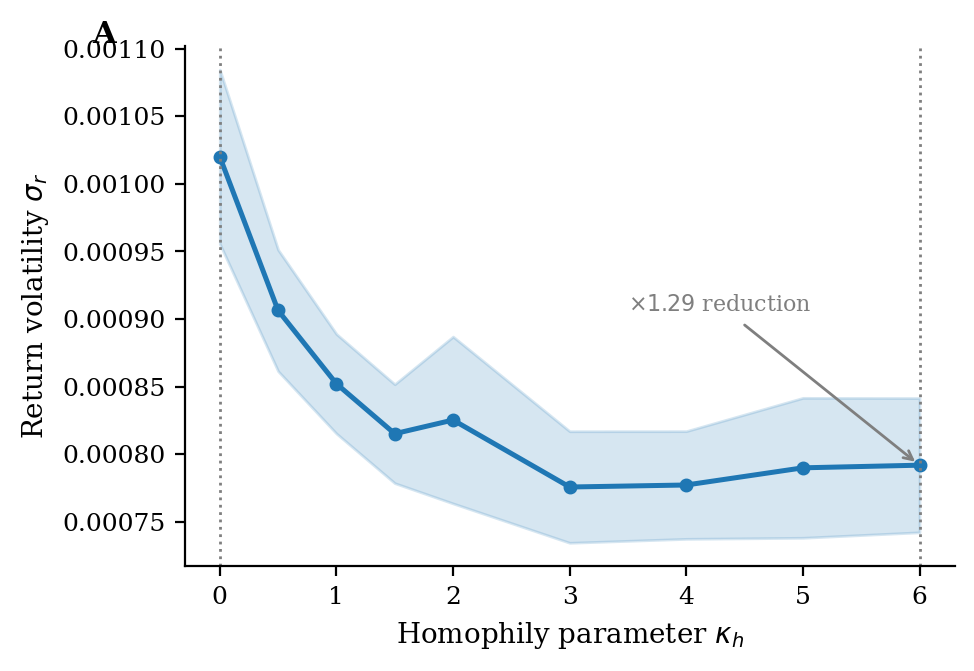
\includegraphics[width=0.85\linewidth]{fig2a}
  \caption{Volatility $\sigma_r$ and TMFI vs.\ $\kappa_h$
  (median $\pm$ IQR, 250 seeds).
  Volatility falls $1.29\times$; TMFI falls $14.28\times$.}
  \label{fig:vol_tmfi}
\end{figure}

\begin{figure}[htbp]
  \centering
  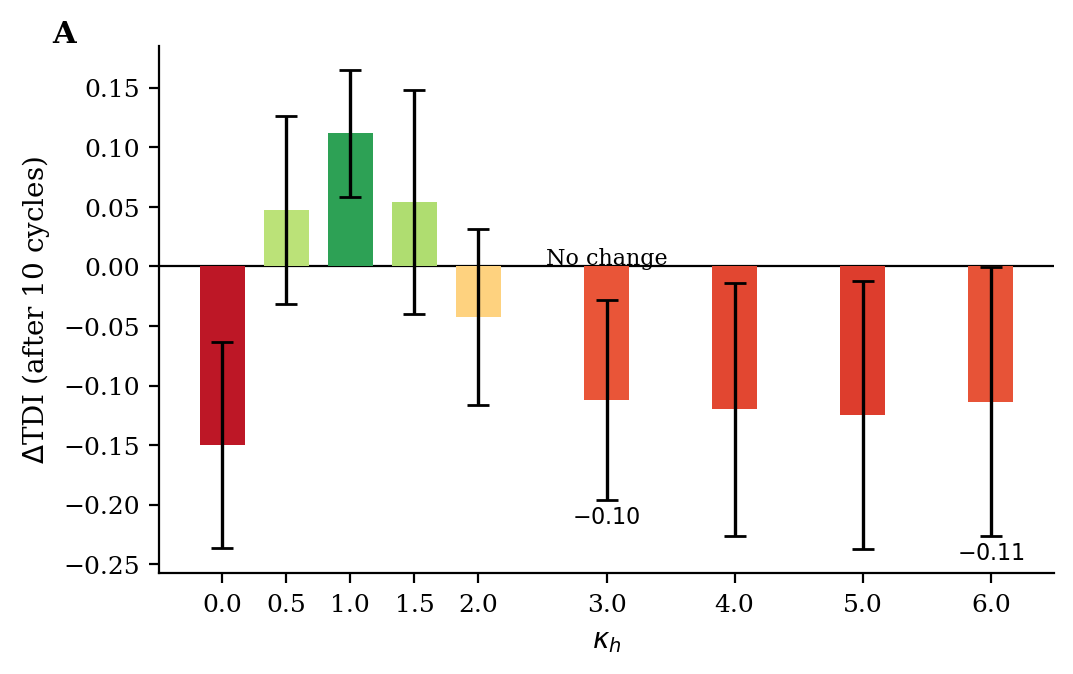
\includegraphics[width=0.85\linewidth]{fig6a}
  \caption{$\Delta$TDI over ten adaptation cycles at
  $\kappa_h \in \{0.5,\,3,\,6\}$:
  $+0.061$, $-0.114$, $-0.102$ respectively.
  Echo-chamber formation is fastest at moderate homophily due to
  bridge connections preserving cross-$\tau$ adaptation pull.}
  \label{fig:deltaTDI}
\end{figure}

\begin{figure}[htbp]
  \centering
  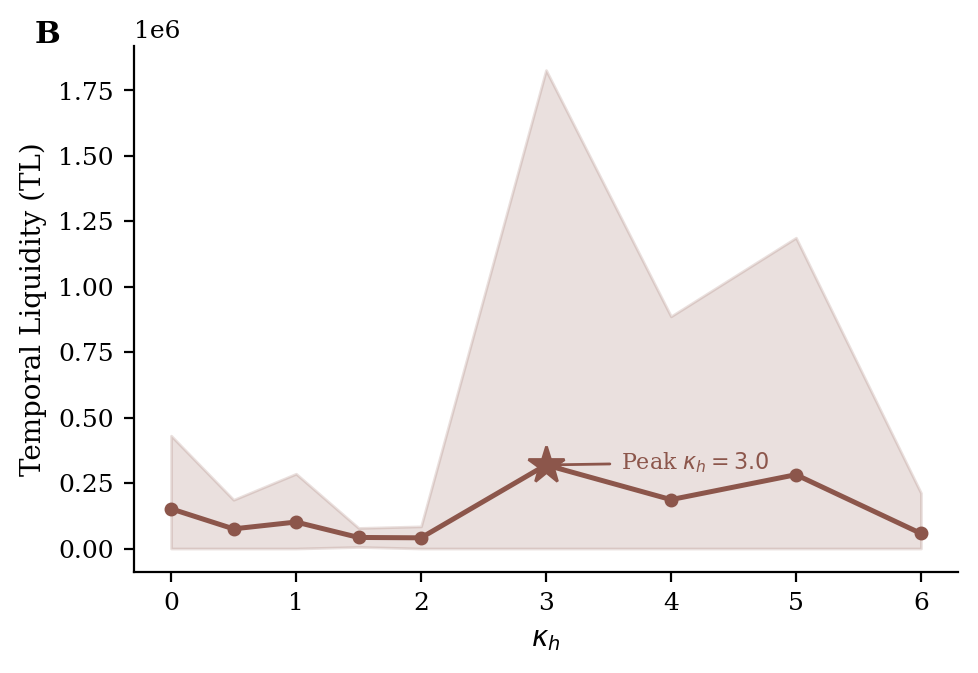
\includegraphics[width=0.85\linewidth]{fig6b}
  \caption{Temporal Liquidity (TL) sweep (50-seed mean $\pm$ std).
  TL peaks at $\kappa_h \approx 3.0$, marking the Goldilocks zone
  where moderate connectivity maximises cross-$\tau$ trade flow before
  $\tau$-cliques fragment the network.}
  \label{fig:TLsweep}
\end{figure}

%% ============================================================
\section{Empirical Validation}
\label{sec:empirical}

We test the CME prediction that high homophily compresses the $\tau$
distribution (low TDI) and is associated with high volatility, using
SEC Form~13-F-HR quarterly institutional holdings data.
Every institutional manager with over \$100~million in qualifying assets
discloses long equity positions quarterly; these filings provide the
most comprehensive available panel of institutional portfolio behaviour
at the frequency and duration required to identify $\tau$.
We use the top~150 filers by historical frequency.
We restrict to quarters with at least 50 reporting institutions, which
excludes 2013~Q1--Q2 where filer coverage was sparse under the
post-XML-standardisation rollout; this yields $n = 45$ quarters
(2013~Q3--2024~Q3).

Each filer's lookback horizon is estimated from quarter-over-quarter
portfolio turnover $\theta_i$ as $\tau_i = 63/\theta_i$, clamped to
$[5,\,1260]$ trading days.
TDI is computed quarterly using $K = 16$ log-$\tau$ bins, matching the
simulation formula exactly.
The quarterly VIX (CBOE) is the volatility proxy.

The principal result:
\[
  r(\mathrm{TDI},\,\mathrm{VIX}) = -0.526,
  \quad p = 0.0002, \quad n = 45.
\]
Higher volatility is associated with compressed $\tau$-diversity---the
empirical analogue of homophily-induced TDI suppression.
TDI drops sharply during crises: 2020~Q1 (COVID-19) registers
$\mathrm{TDI} = 1.550$; 2022~Q4 (Fed tightening, FTX collapse) reaches
the sample minimum $\mathrm{TDI} = 1.021$.
Calm bull markets show high TDI: 2024~Q1 reaches $1.980$ and 2017~Q4
reaches $1.971$.
Excluding 2022~Q4 as a candidate outlier, the correlation is
$r = -0.393$ ($p = 0.0075$), confirming the result is not driven by a
single observation.
An exploratory lagged specification finds
$r(\mathrm{VIX}[t],\,\mathrm{TDI}[t+1]) = -0.298$ ($p = 0.047$),
suggestive of institutional inertia; this does not survive
Bonferroni correction and is treated as exploratory.

\begin{figure}[htbp]
  \centering
  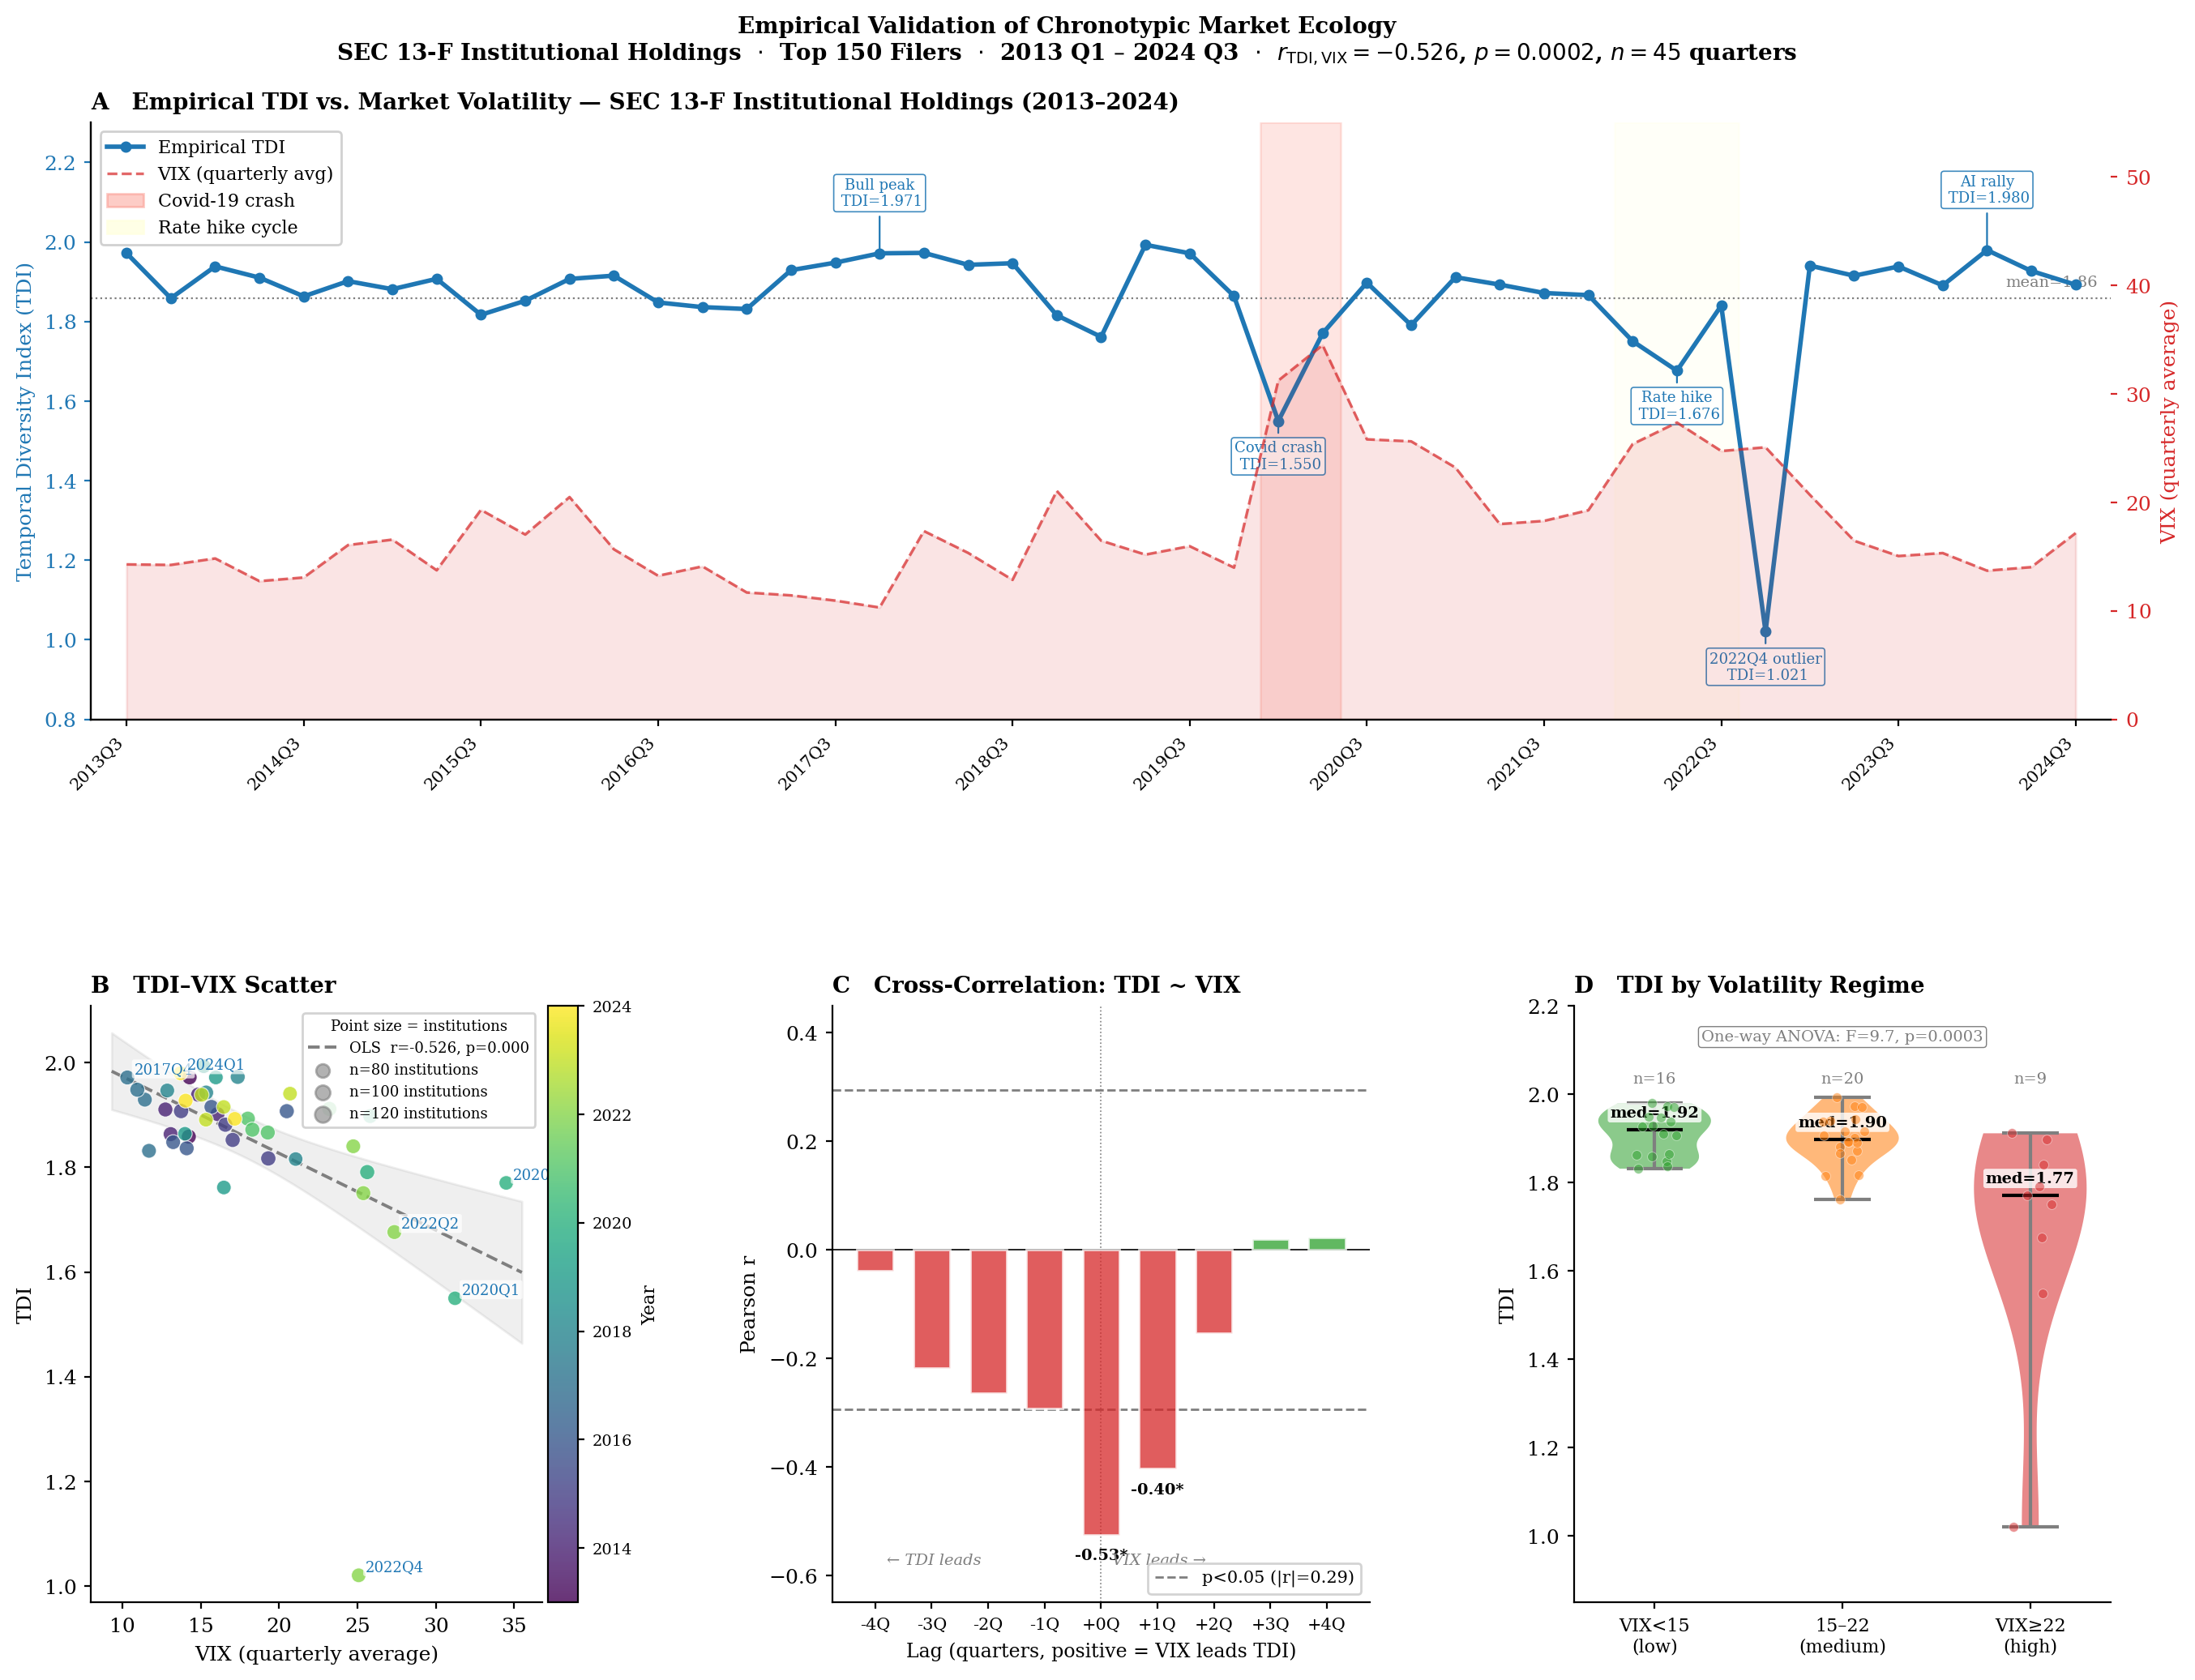
\includegraphics[width=\linewidth]{empirical_tdi_validation}
  \caption{Top: Empirical TDI (blue) vs.\ quarterly VIX (red dashed),
  2013--2024.  Shaded: COVID-19 crash (2020~Q1--Q2) and Fed rate-hike
  cycle (2022~Q1--Q3).  Bottom left: TDI--VIX scatter; OLS fit
  $r = -0.526$, $p < 0.001$.  Bottom right: cross-correlation function
  at lags $k \in \{-2,\ldots,+2\}$ quarters.}
  \label{fig:empirical}
\end{figure}

\paragraph{Interpretation.}
The empirical pattern maps directly onto the CME mechanism.
The simulation predicts that high homophily pressure compresses the $\tau$
distribution and reduces TDI; the 13-F evidence suggests that high-volatility
environments generate an analogous exogenous compression.
During crises, institutions that outperform tend to be those with
short-horizon positions, and others rebalance toward similar horizons,
crowding the $\tau$ distribution and driving TDI downward.
In low-volatility bull markets, by contrast, longer-horizon investors can
profitably hold positions across a wider range of $\tau$ values, allowing
TDI to re-expand.
This interpretation is consistent with the one-quarter lag finding
($r = -0.298$, $p = 0.047$): even after volatility subsides, portfolios
take time to re-diversify, a temporal analogue of the institutional inertia
embedded in the model's $\tau$-adaptation rule.

\paragraph{Limitations of the empirical analysis.}
Turnover is a noisy proxy for $\tau$: derivatives positions are not
captured, quarterly reporting misses intra-quarter adjustments, and the
inverse-proportionality mapping $\tau_i = 63/\theta_i$ imposes a
functional form that may not hold uniformly across institution types.
Restricting to long equity positions in 13-F filings understates the full
breadth of horizon heterogeneity; hedge funds with large short books are
particularly underrepresented.
Despite these limitations, the consistency of sign, magnitude, and lag
structure with the CME simulation provides meaningful out-of-sample
support for the framework's core mechanism.

%% ============================================================
\section{Discussion and Conclusion}
\label{sec:conclusion}

CME provides a network-based microfoundation for the Fractal Market
Hypothesis \citep{peters1994} and extends it with a dual-channel dynamic.
The \emph{short-run stabilising channel}: high temporal homophily suppresses
aggregate volatility $1.29\times$ ($t = 15.1$, $p < 10^{-20}$) and nearly
eliminates temporal fragmentation (TMFI falls $14.28\times$) by clustering
like-horizon agents and reducing cross-$\tau$ friction.
The \emph{long-run destabilising channel}: $\tau$-adaptation under high
homophily is self-reinforcing ($\Delta\mathrm{TDI} = -0.114$ at
$\kappa_h = 3.0$ over ten cycles), collapsing the horizon diversity that
the FMH identifies as the foundation of market stability.
SEC~13-F data ($r = -0.526$, $p < 0.001$, $n = 45$ quarters) confirm the
long-run channel: high-volatility environments are associated with
compressed institutional horizon diversity, consistent with the echo-chamber
mechanism operating over medium-to-long horizons.

Three limitations circumscribe these conclusions.
First, the TMFI ratio has substantial seed-level variance; the $14.28\times$
figure is a 30-seed mean that requires further robustification, particularly
under alternative network formation rules.
Second, the turnover-to-$\tau$ mapping $\tau_i = 63/\theta_i$ is a noisy
proxy that cannot recover intra-quarter horizon shifts or derivative positions.
Third, $\kappa_h$ is an exogenous parameter; a structural identification
strategy from trade-level or order-flow data would substantially strengthen
the empirical grounding.

The most productive extensions are: (a) endogenising the $\tau$ distribution
via rational inattention \citep{sims2003}, in which capacity-constrained
agents optimally specialise in return frequencies so the $\tau$ distribution
emerges as equilibrium; (b) developing observable proxies for TMFI and TL
that can be computed from transaction-level data; and (c) testing whether
the non-monotonic echo-chamber speed result holds in richer models with
strategic agents.
On the policy side, the Goldilocks finding---Temporal Liquidity peaks at
moderate homophily---suggests that market designs preserving diverse-horizon
participation reduce the risk of self-reinforcing chronotypic convergence
during stress events, when the CME model predicts the strongest echo-chamber
formation pressure.
Whether regulatory instruments such as cross-horizon market-maker
obligations or $\tau$-diversity disclosure requirements can shift
$\kappa_h$ toward this optimal zone is a question for future empirical work.

%% ============================================================
\section*{Acknowledgements}

We thank Professor Andrew Caplin (New York University) for helpful comments and suggestions.

%% ============================================================
\section*{Funding}

This research did not receive any specific grant from funding agencies
in the public, commercial, or not-for-profit sectors.

%% ============================================================
\section*{CRediT author contribution statement}

\textbf{Sanjay Subramanian:} Conceptualization, Methodology, Software,
Formal analysis, Data curation, Writing---original draft,
Writing---review and editing.
\textbf{Sumedh Seetharaman:} Conceptualization, Methodology,
Formal analysis, Validation, Writing---review and editing.

%% ============================================================
\section*{Declaration of competing interest}

The authors declare that they have no known competing financial interests
or personal relationships that could have appeared to influence the work
reported in this paper.

%% ============================================================
\section*{Data availability}

Simulation code (Python 3.11+), parameter files, and generated figures
are available at \url{https://doi.org/10.5281/zenodo.21408851}.
SEC Form~13-F data were retrieved from the EDGAR full-text search system;
the processed quarterly TDI series is included in the repository.

%% ============================================================
\section*{Declaration of generative AI and AI-assisted technologies
          in the manuscript preparation process}

During the preparation of this work, the authors used Claude (Anthropic)
to assist with LaTeX typesetting, code debugging, and draft revision.
After using this tool, the authors reviewed and edited all content and
take full responsibility for the content of this publication.

%% ============================================================
\bibliographystyle{elsarticle-harv}

\begin{thebibliography}{15}

\bibitem[Acemoglu et al.(2015)]{acemoglu2015}
Acemoglu, D., Ozdaglar, A., Tahbaz-Salehi, A., 2015.
Systemic risk and stability in financial networks.
\textit{American Economic Review} 105 (2), 564--608.

\bibitem[Allen and Gale(2000)]{allen2000}
Allen, F., Gale, D., 2000.
Financial contagion.
\textit{Journal of Political Economy} 108 (1), 1--33.

\bibitem[Arthur et al.(1997)]{arthur1997}
Arthur, W.B., Holland, J.H., LeBaron, B., Palmer, R., Tayler, P., 1997.
Asset pricing under endogenous expectations in an artificial stock market.
In: Arthur, W.B., Durlauf, S.N., Lane, D.A. (Eds.),
\textit{The Economy as an Evolving Complex System~II}.
Addison-Wesley, pp.\ 15--44.

\bibitem[Bikhchandani et al.(1992)]{bikhchandani1992}
Bikhchandani, S., Hirshleifer, D., Welch, I., 1992.
A theory of fads, fashion, custom, and cultural change as informational
cascades.
\textit{Journal of Political Economy} 100 (5), 992--1026.

\bibitem[Caplin and Dean(2015)]{caplin2015}
Caplin, A., Dean, M., 2015.
Revealed preference, rational inattention, and costly information acquisition.
\textit{American Economic Review} 105 (7), 2183--2203.

\bibitem[Cont(2001)]{cont2001}
Cont, R., 2001.
Empirical properties of asset returns: stylized facts and statistical issues.
\textit{Quantitative Finance} 1 (2), 223--236.

\bibitem[Corsi(2009)]{corsi2009}
Corsi, F., 2009.
A simple approximate long-memory model of realized volatility.
\textit{Journal of Financial Econometrics} 7 (2), 174--196.

\bibitem[Devenow and Welch(1996)]{devenow1996}
Devenow, A., Welch, I., 1996.
Rational herding in financial economics.
\textit{European Economic Review} 40 (3--5), 603--615.

\bibitem[Elliott et al.(2014)]{elliott2014}
Elliott, M., Golub, B., Jackson, M.O., 2014.
Financial networks and contagion.
\textit{American Economic Review} 104 (10), 3115--3153.

\bibitem[Farmer and Foley(2009)]{farmerfoley2009}
Farmer, J.D., Foley, D., 2009.
The economy needs agent-based modelling.
\textit{Nature} 460 (7256), 685--686.

\bibitem[Golub and Jackson(2012)]{golub2012}
Golub, B., Jackson, M.O., 2012.
How homophily affects the speed of learning and best-response dynamics.
\textit{Quarterly Journal of Economics} 127 (3), 1287--1338.

\bibitem[LeBaron(2001)]{lebaron2001}
LeBaron, B., 2001.
A builder's guide to agent-based financial markets.
\textit{Quantitative Finance} 1 (2), 254--261.

\bibitem[M{\"u}ller et al.(1993)]{muller1993}
M{\"u}ller, U.A., Dacorogna, M.M., Dav{\'e}, R.D., Olsen, R.B.,
Pictet, O.V., von Weizs{\"a}cker, J.E., 1993.
Fractals and intrinsic time---a challenge to investment managers.
\textit{Olsen \& Associates Preprint}, Zurich.
Reprinted in \textit{Finance}, 1997.

\bibitem[Peters(1994)]{peters1994}
Peters, E.E., 1994.
\textit{Fractal Market Analysis: Applying Chaos Theory to Investment and
Economics}.
Wiley Finance Editions, New York.

\bibitem[Peng and Xiong(2006)]{peng2006}
Peng, L., Xiong, W., 2006.
Investor attention, overconfidence and category learning.
\textit{Journal of Financial Economics} 80 (3), 563--602.

\bibitem[Sims(2003)]{sims2003}
Sims, C.A., 2003.
Implications of rational inattention.
\textit{Journal of Monetary Economics} 50 (3), 665--690.

\end{thebibliography}

\end{document}
